\documentclass[preprint]{iucr}
 \journalcode{J}
 \papertype{CP}

\usepackage{graphicx}

\usepackage[T1]{fontenc}
\usepackage[utf8]{inputenc}

\begin{document}

\title{The Fast Azimuthal Integration Python library}
\shorttitle{PyFAI}

    \author[a]{Aurore}{Deschildre}
    \author[a]{Giannis}{Ashiotis}
    \author[b]{Zubair}{Nawaz}
    \author[a]{Jonathan P.}{Wright}
    \author[c]{Fr\'ed\'eric-Emmanuel}{Picca}
    \cauthor[a]{J\'er\^ome}{Kieffer}{jerome.kieffer@esrf,fr}{}
    \aff[a]{European Synchrotron Radiation Facility, \city{Grenoble}, \country{France}}
    \shortauthor{Kieffer et al.}

\maketitle

\begin{synopsis}

\end{synopsis}

\begin{abstract}
\end{abstract}

\section{Introduction}

\subsection{Experiment description}
In pyFAI, a basic experiment is defined by an area-detector which position in
space is defined versus the intersection of the incoming pencil beam and the
sample plan.

\subsection{Detector}
Like most other image processing packages, pyFAI allows the definition of 2D
detectors by the pixel size (in meter) but shows its limits with modern pixel
detectors.

\subsubsection{Detectors classes}
Large area pixel detector are often composed from the assembly of smaller
modules. Often such detector exhibit gaps beteween modules and pixels of various
sizes within a module, hench requires a specific mask.
To take the specificites of each detector into account, pyFAI contains about
40 detectors class definition which contains the mask (invalid pixels, gaps,
\ldots) and a method to calculate the pixel positon in cartesian coordinates.

\subsubsection{Nexus Detectors}
Optically coupled CCD detector and Pilatus detectors should also be corrected
for small spacial displacement of the pixel, often called geometric distortion.
Any detector object in PyFAI, can be saved to a HDF5 file
following the NeXus conversion (slightly modified).
Detector objects can then be restored from the disk, making detector definition
less error-prone.
Pixels of a 2D detector are saved as a 4D HDF5-dataset: 2D array of vertices
pointing to every corner of each pixel, which makes an array of shape: (ny, nx, 4, 3)
This can define detectors no longer planar, like tiled detectors from
ImXpad or the Pilatus12M from Dectris, even accounting for the normal of each
pixel.

\subsection{Geometry}
The experiment geometry is defined in pyFAI by six parameters: the sample
detector distance along with the detector coordinates of the sample's ortohgonal
projection on the detector plane, called PONI. The detector's rotation along the
three axes are completing those six parameters. All three distances are handeled
as meter and all three rotation are given in radians. Those S.I. units may look
unadapted and odd to users familliar to other code like FIT2D \cite{fit2d},
therefore the geometry can be exported to (or imported from) other software.   

 
\subsubsection{Binning}
One of the strength of this geometry is capability to perform binning of the
detector without having to re-calibrate or re-calculate the position in space.
All pyFAI detector classes have a binning option which will increase the pixel
size accordingly and divide detector shape accordingly.

\section{Calibration}
Calibration of the position of the detector is performed using Debye-Scherrer
rings collected from a reference powder called ``calibrant''.
Rings are extracted and control points are located as maxima of those rings.
The geometry of the experiment is obtained from a least-squares refinement of
the $2\theta$ angles.

\subsection{Calibrant}
PyFAI provides ten calibrants files among the most used ones: ceria, corundum,
gold, lantahnide hexaboride and silicon for powder diffraction; silver behenate,
tetradecanol and para-bromobenzoic acid for small angle scattering.
Any file containing d-spacing in angstrom can be used as calibrant for a
geometry calibration and will be loaded by the $Calibrant$ class.
This class,
together with the provided wavelength provide the reference $2\theta$ position
against which the geometry will be refined.

\subsection{Peak-picking}

\subsubsection{Massif}
\subsubsection{blob detection}
\subsection{User interface}

\section{Integration}
\subsection{Pixel splitting schemes}
\subsubsection{No splitting}

TODO \ldots \cite{bilinge2014}

\subsubsection{Bounding box splitting}
\subsubsection{Tight pixel splitting}
\subsubsection{Pixel correlation}
\subsection{User interface}

\section{Signal separation}
\subsection{Diffraction image generation}

As an azimuthal integrator object knows about the position of the detector in
space, hence the $2\theta$ and $\chi$ position of every single pixel, it is not
only able to perform averaging and regrouping  but also to
reconstruct various types of images assuming an azimuthal symmetry.
#: simulated
#2D diffraction patterns (mainly for testing) but also from actual signal.
This method, $calcfrom1d$, is for example used together with a calibrant object
to generate a fake diffraction image suitable for testing pyFAI or other
calibration codes (for example to validate the geometry translation from one
program to another).

\subsection{Image offset and validation of the calibration}
By regenerating a 2D diffraction image from the integrated powder pattern one
can assess the quality of the calibration used for the integration.
The calibration tool, pyFAI-calib, offers  a ``validate'' command which measures
the offset on the image (x, y) between the 2D diffraction image and the one
regenerated from the integrated patern, using a phase correlation algorithm.
This allows a measurement of the precision of the PONI, which is often better
than a tenth of a pixel !
To obtain such a result, a proper calibration image with continuous rings (i.e.
not spotty) and a mask to remove the beam stop are mandatory.

\subsection{Amorphous background removal}

PyFAI's azimuthal integrator features a $separate$ method able to separate
the backgound with an azimuthal symmetry (amorphous scattering or powder ring),
from Bragg peaks automatically.

Based on what was described in \cite{PyFAI_PDJ}, a bidimentional azimuthal
integration is performed on the input image.
The output 2D image is filtered out along the azimuthal $\chi$ axis using a
percentile filter to construct the powder diffraction curve without the punctual
Bragg spots.
The number of points in azimuthal and radial direction as well as
the percentile value can be adjusted but the default values are reasonnably
good.

The reconstructed 2D image corresponds to the amorphous/powder/isotropic
composant of the input image and the subtraction of this generated image from
the raw data contains only the bragg signal.
Figure \ref{separate} (left)
presents a close-up look at the first image of a Lysozyme dataset provided by Dectris to
advertize their Pilatus 6M detectors (image taken at the Swiss Light Source). A
moderate ice-ring is clearly visible. After using the automatic amorphous
background removal, which takes into account the mask needed for such pixel
detector, only Bragg peaks remains (right of the image).

\begin{figure}
\label{separate}
\begin{center}
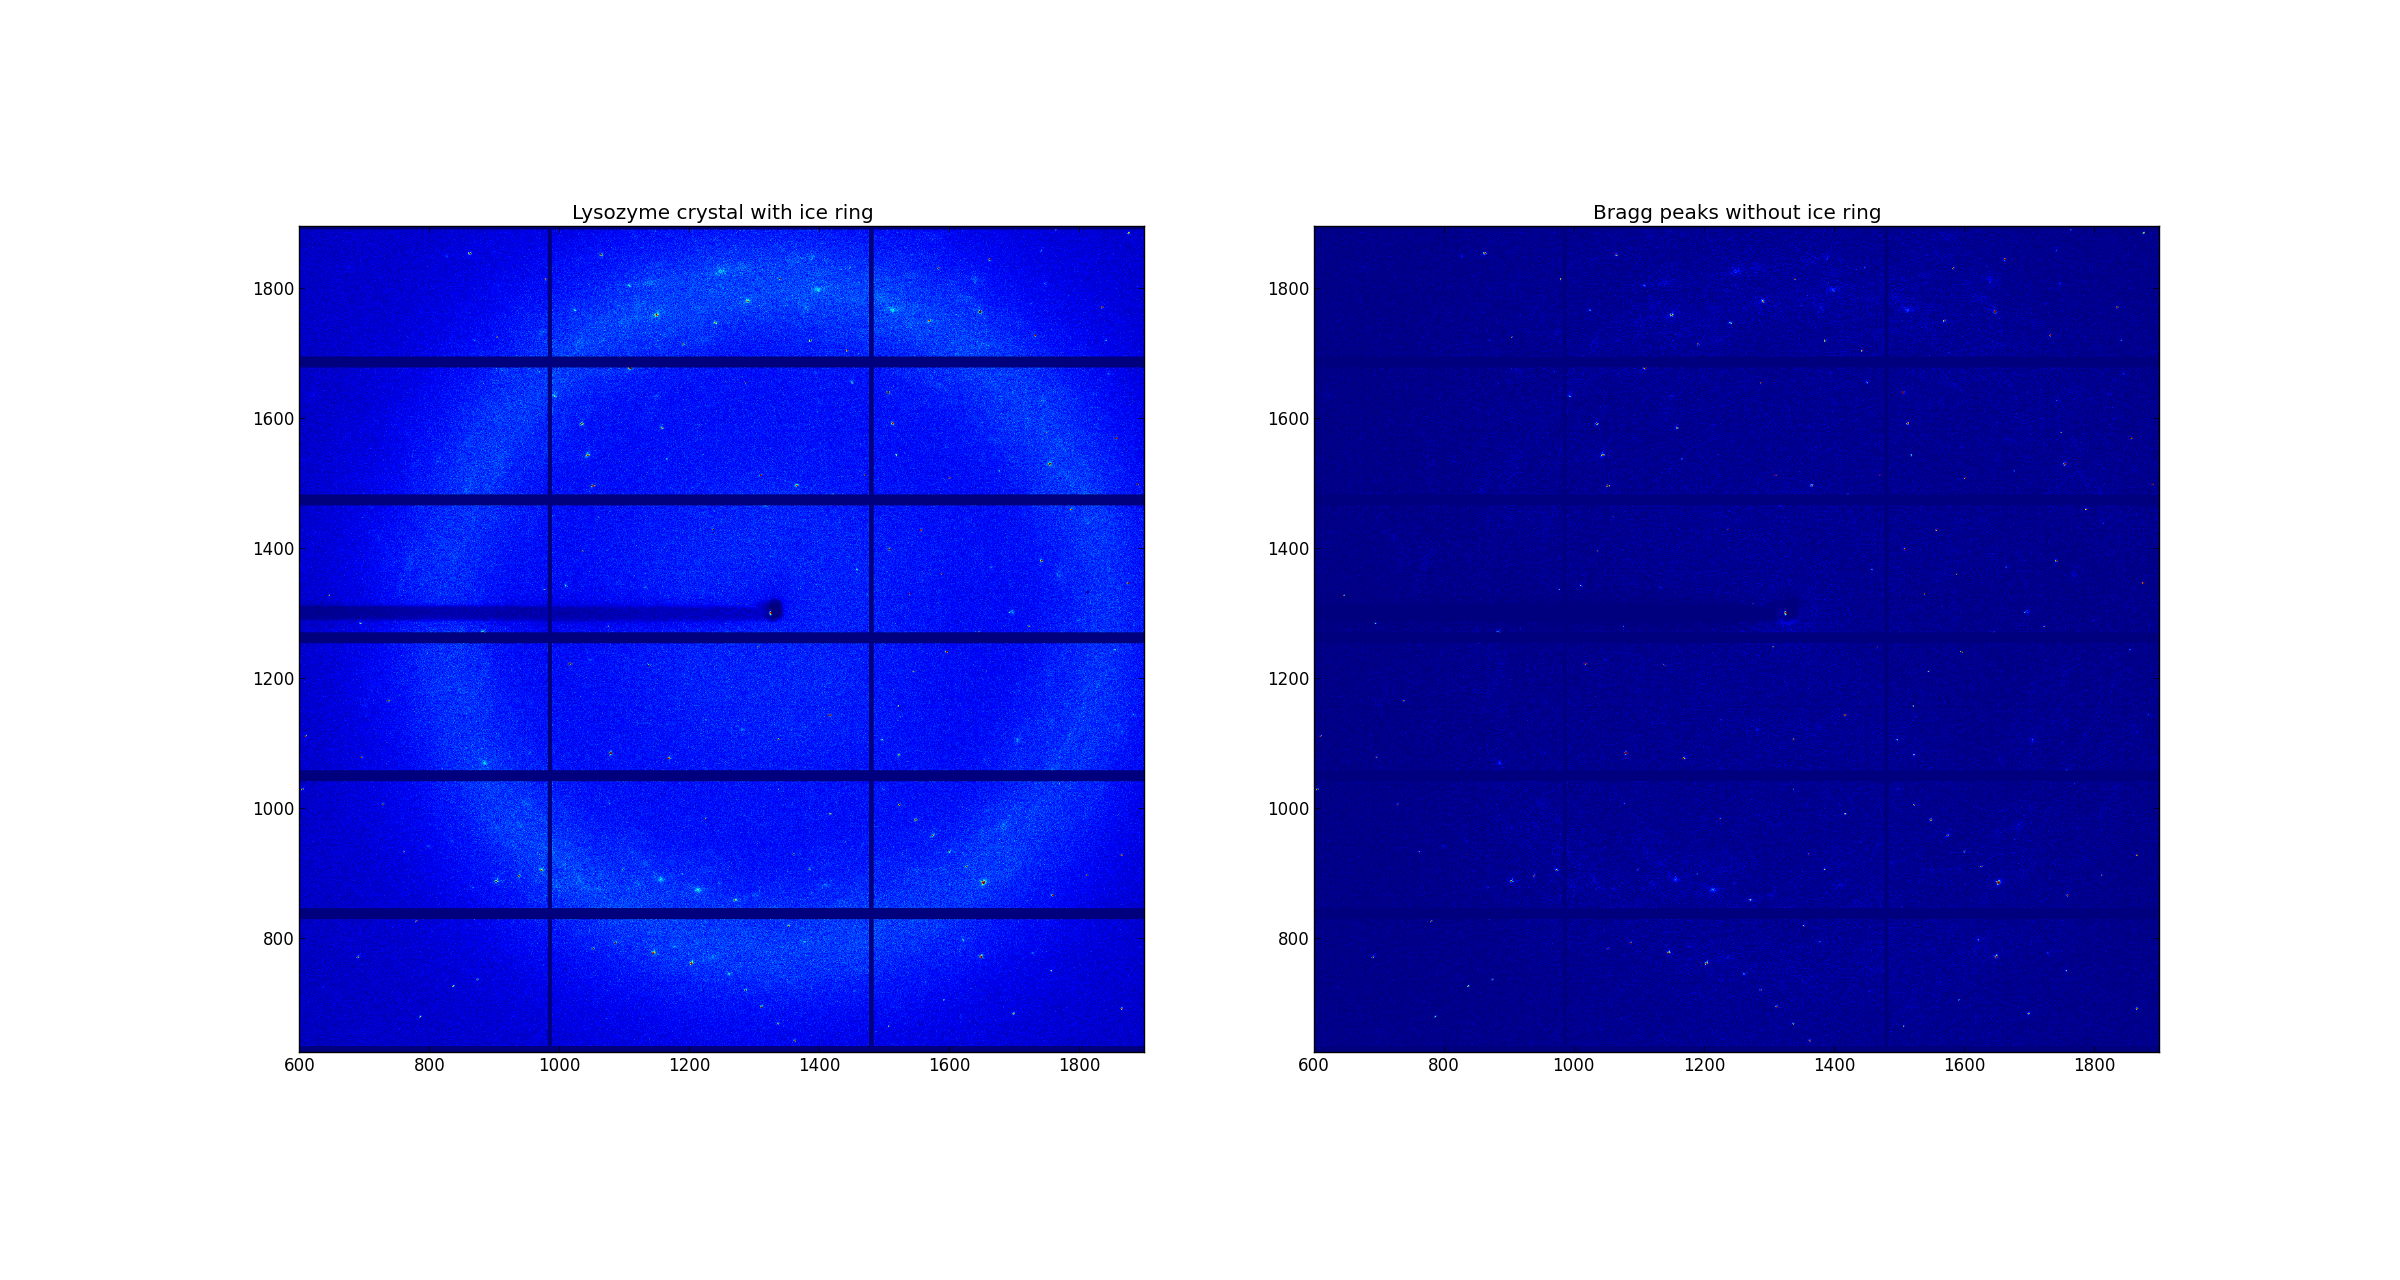
\includegraphics[width=15cm]{separate.eps}
\caption{Automatic separation of amorphous signal from Bragg peaks in a
protein crystallography experiment.}
\end{center}
\end{figure}

\subsubsection{Application to high-pressure diffraction}
When high-pressure diffraction is performed using diamond anvil cells, the Bragg
reflection from diamond tend to polluted the powder diffraction signal. PyFAI's
isotropic component separation can also be used to retieve the powder signal and
discard the signal from the the diamond.

\subsubsection{Application to serial crystallography}
In those experiment, tiny crystals in their medium (liquid) are sent in front of
the X-ray beam (using a jet or moving a motor) and data are acquired
continuously, using a fast detector (from dozens of Hertz to kHz).
Those experiment produce a huge amount of data and only a small fraction of the
frames contain actually diffraction signal.
PyFAI, when integrated into the LImA data acquisition system \cite{lima},
can be used to assess the amount of single crystall diffraction data and decide
to save or not any frame, saving a huge amount of disk space and network
bandwidth.



\section{Conclusion}




\bibliographystyle{iucr}
\bibliography{biblio}
\appendix
\section{Project structure}
PyFAI is an open source project licensed under the GPL mainly written in Python (v2.6 or 2.7)
and heavily relying on the python scientific ecosystem: NumPy, SciPy and Matplotlib.
It provides high performances image treatment thanks to Cython and PyOpenCL.

The project is hosted on GitHub (https://github.com/kif/pyFAI) which provides
the issue tracker in addition to code hosting.
To ease the distribution, the
software is available as official Debian package and included in some of the
most famous linux distribution like Ubuntu and Debian.
The program runs also on other operating systems like Windows and MacOSX.

Anybody can fork the project and adapt it to his own needs: CEA-saclay,
Synchrotrons Soleil and APS did it. If developments are useful to be shared,
they can be merged into the main branch via pull-requests.

\section{Parallel implementations using OpenCL}
Azimuthal integration and many other computing parts in pyFAI were written in
OpenCL kernels and interfaced using PyOpenCL \cite{pyopencl}. PyOpenCL offers a
shared execution model effective both on processors (CPU), graphics cars (GPU)
and accelerators like the Intel's Xeon Phi.

\subsection{Azimuthal Integration}
The direct azimuthal integration is basically a scatter operation which
requires large locked section.
To overcome this limitation, pixels have been
associated to the output bin of the histogram and stored in a look-up
table (LUT), making the integration look like a simple (if large and sparse)
matrix vector product.
The sparse matrix ``Compressed Sparse Row'' (CSR) format is now used in pyFAI,
saving about half of the space of the LUT previously used.
Secondly, all threads within a workgroup are collaborating to calculate the
matrix-vector product via a so-called ``parallel reduction'', offering
additional speed-up (especially on GPUs).
The compensated algebra (Kahan summation) is kept to maintain the precision
of the calculation while using single precision (32 bits) floating points
arithmetics.

\subsection{Look-up table creation}


\ack{Acknowledgements}

The author would like to thank all ESRF beamline teams for \ldots

In the instrumentation division (ISDD) we would like to thank Claudio Ferrero,
head of data analysis unit, and Andy G\"otz, head of software group, for
supporting the parallelization work on the presented algorithm.
V. Armando Solé, the author of PyMca, is also acknowledged for providing a

LinkSCEEM \ldots



\end{document}
